\documentclass[11pt,a4paper]{article}
% Encoding and language
\usepackage[utf8]{inputenc}
\usepackage[english]{babel}
% Colors
\usepackage[usenames,dvipsnames]{color}
\usepackage{colortbl}
% Paper size and margins
\usepackage{vmargin}
\setmarginsrb{2cm}{2cm}{2cm}{2cm}{0cm}{0cm}{0cm}{1.5cm}
% Indenting
\usepackage{indentfirst}
%\setlength{\parindent}{1cm}
\setlength{\parskip}{0.5cm}
% Symbols
\usepackage{amsmath}
\usepackage{amsfonts}
\usepackage{amssymb}
% Equations
\usepackage{eulervm} % upright font in eqns (Palatino)
\usepackage{cool}
\usepackage{mathtools} % for arrows
% References
\usepackage{natbib}
\bibliographystyle{apalike}
% Hyperlinks and labels
%\usepackage{showkeys}
\usepackage[linktocpage=true,plainpages=false,pdfpagelabels=false]{hyperref}
\definecolor{citecolor}{rgb}{0.2,0.7,0.9}
\definecolor{urlcolor}{rgb}{0,0,1}
\hypersetup{
    colorlinks, linkcolor={Black},
    citecolor={Black}, urlcolor={Black}
}
% Figures
\usepackage{subcaption}
\usepackage{tikz}
\usetikzlibrary{shapes,arrows}
\usetikzlibrary{positioning}
\usetikzlibrary{calc}
% Tikz styles
\tikzstyle{reg} = [rounded rectangle, text width=2cm, fill=black!5, align=center, anchor=west,font=\sffamily\Large\bfseries, minimum height=1cm, inner sep=0]
\tikzstyle{rad} = [rounded rectangle, draw=none, text width=2cm, fill=red!10, align=center, anchor=west,font=\sffamily\Large\bfseries, minimum height=1cm, inner sep=0]
\tikzstyle{long} = [rounded rectangle, draw=none, text width=3.5cm, fill=black!5, align=center, anchor=west,font=\sffamily\Large\bfseries, minimum height=1cm, inner sep=0]   
\tikzstyle{add} = [scale=1.5, draw=none,fill=none,align=center]
\tikzstyle{emp} = [draw=none,fill=none]
\tikzstyle{ar} = [->,draw=black!70,line width=2]
\tikzstyle{ln} = [-,draw=black!70,line width=2]
% Title etc
\newcommand{\mytitle}{Analysis of the Relationships between Alkyl Nitrates and Their Parent Hydrocarbons}
\newcommand{\authorname}{Maria Zamyatina}
\newcommand{\univname}{University of East Anglia}
\newcommand{\facname}{School of Environmental Sciences}
\newcommand{\mydate}{\the\year}
% Remove author and date from the maketitle command
\makeatletter
\renewcommand{\@maketitle}{
\newpage
 \null
 \vskip 2em%
 \begin{center}%
  {\LARGE \@title \par}%
 \end{center}%
 \par} \makeatother
% PDF meta-data
\hypersetup{pdftitle={\mytitle}}
\hypersetup{pdfauthor=\authorname}

\title{\mytitle}
% =========================================================================
\begin{document}
\maketitle

\begin{abstract}
This work is based on alkyl nitrate measurements from four field campaigns, from ground-based sites across the British Isles and aircraft measurements over the North Atlantic. The ratios between the alkyl nitrates and their parent hydrocarbons are compared with those expected from the photochemical theory. The sensitivity analysis to the theoretical assumptions and uncertainties in measurements revealed a good general agreement between observed and theoretical data.
\end{abstract}
\smallskip
\noindent \textbf{Keywords:} alkyl nitrate, parent hydrocarbon, NAMBLEX, ITOP, TORCH

\section{Introduction} \label{sec:intro}
Alkyl nitrates ($RONO_2$) are organic tropospheric trace gases. They are produced photochemically through the oxidation of their parent hydrocarbons \citep{Roberts1990} or emitted directly from equatorial oceans \citep{Blake2003} and biomass burning \citep{Simpson2002}. Being involved in the ozone production chemistry, these species can act as reservoirs of nitrogen oxides which availability largely affects the production of ozone \citep{Reeves2007}. Since the alkyl nitrates have atmospheric lifetimes ranging from several days to about a month, they can redistribute nitrogen oxides presented over polluted continental regions to clean remote marine environments, and therefore are considered as one of the tracers for determining the anthropogenic influence \citep{Atherton1989, Reeves2007, Worton2005}.

Alkyl nitrates are removed from the atmosphere by photolysis \citep{Turberg1990} or through oxidation by hydroxyl radical ($OH$) \citep{Talukdar1997}. Photolysis is the dominant loss mechanism for the compounds with short carbon chains and becomes more important with decreasing carbon number. Reaction with $OH$ follows the opposite trend and is most important for the pentyl nitrates and higher.

Owing to the existence of the relationship between alkyl nitrates and their parent hydrocarbons, measurements of their concentrations can provide information on the extent of photochemical processing in the air mass. \cite{Bertman1995} developed a kinetic approach to describe this relationship through the evolution of the ratio of alkyl nitrate to its parent hydrocarbon as a function of time. This approach has been extensively used to study air mass photochemical ageing at several sites, in North America \citep{Bertman1995, Roberts1998}, China \citep{Simpson2006}, the British Isles \citep{Worton2010} and over the Pacific \citep{Simpson2003} and North Atlantic Ocean \citep{Reeves2007}.

\cite{Bertman1995} found that the theoretical ratios of  2-butyl nitrate to n-butane and 2- and 3-pentyl nitrates to pentane strongly agree with those measured from the ambient air showing no evidence for primary sources of these nitrates. On the contrary, measurements of the other ratios, ethyl/ethane, n-propyl nitrate/propane, and 2-propyl nitrate/propane, appeared to be significantly higher than predicted, relative to the 2-butyl nitrate/n-butane ratio, meaning that there should be an additional source of these alkyl nitrates. \cite{Roberts1998} generally approved the theory by comparing Bertman's conclusions with the results from a new observational dataset.

Using methyl nitrate as a tracer of marine $RONO_2$ \cite{Simpson2006} revealed that the South China Sea in not a region of strong $RONO_2$ emissions suggesting that photochemical rather marine production of alkyl nitrates is dominant at the site.

\cite{Worton2010} found that the photochemical source of the short-chain alkyl nitrates originates mostly from the photochemical oxidation and decomposition of longer-chain compounds rather than from the oxidation of the parent hydrocarbons as it is thought in the previous studies.

In order to extend our understanding of the photochemical processing of the air the present work compares theoretical results of \cite{Bertman1995} with those calculated from recent alkyl nitrate data of four field campaigns, namely the North Atlantic Marine Boundary Layer Experiment (NAMBLEX), the Intercontinental Transport of Ozone and Precursors (ITOP) and two Tropospheric Organic CHemistry experiments (TORCH1 and TORCH2). The brief description of the measurement sites and data is presented in section \ref{sec:data}. In section \ref{sec:method} the methodology used in this work is defined. Section \ref{sec:res} contains the results. Section \ref{sec:discuss} discusses the results, particularly focusing attention on the analysis of the discrepancy between the observational data and the results of theoretical modelling. Conclusions constitute section \ref{sec:conclusion}.

\section{Data} \label{sec:data}
The data used in this work were collected from tree ground-based and one aircraft campaign at different times of the year and using different methods. Such a variety of data are used in order to compare theoretical conclusions with observational data under a greater variety of atmospheric conditions (than it is possible using only one dataset). It is also allowing us to make a broader sensitivity and uncertainties analysis.

The data of the Tropospheric ORganic CHemistry experiment 1 (TORCH1) were collected at Writtle Colledge, near Chelmsford ($52^\circ N$, $0^\circ E$), Essex, between the 25\textsuperscript{th} July and the 30\textsuperscript{th} August 2003 \citep{Emmerson2007}. The measurement site was located 2 miles west of Chelmsford and 25 miles north east of London thus giving the opportunity to sample recent out flowing air from the London area.

The data of the second such experiment, TORCH2, were collected between April and May 2004 at Weybourne Atmospheric Observatory ($52^\circ N$, $1^\circ E$), which is located on the north Norfolk shore near Weybourne \citep{Gysel2007}. Air masses encountered at this station represent down flow from London, when the prevailing large scale wind direction is south, but when the winds are western or eastern the air comes from the West Midlands or the European continent respectively. When northern winds dominate relatively clean air masses are transported from the North Sea region to the site.

The data of the North Atlantic Marine Boundary Layer Experiment (NAMBLEX) campaign were collected at the Mace Head Atmospheric Research Station in County Galway, Ireland ($53^\circ N$, $10^\circ W$) between the 23\textsuperscript{th} August and the 4nd September 2002 \citep{Heard2006}. This site receives air from a wide range of sources, but mainly is characterised by conditions of exceptionally clean air coming from the Azores and Greenland. The prevailing wind direction ranges from south to north-west meaning that the air has often travelled over the Atlantic Ocean for the five days before its arrival at Mace Head. That is why this site is usually considered representative of background conditions for the Northern Hemisphere.

The last dataset used in this study is the airborne observations made during the Intercontinental Transport of Ozone and Precursors (ITOP) project \citep{Lewis2007b}. These data were collected on board the UK BAe-146 aircraft, which was based at Horta ($38^\circ N$, $28^\circ W$) on the island of Faial, a part of the Portuguese Azores archipelago.

\section{Methodology} \label{sec:method}
Below is the simplified scheme of atmospheric hydrocarbon oxidation leading to the formation of alkyl nitrates (see also Fig. \ref{fig:scheme_bertman}). It begins from the process of $H$ abstraction by the $OH$ radical where the fraction of the primary or secondary radical is denoted by $\alpha_1$.
\begin{equation} \label{eq:alkane_oh}
RH + \bullet OH \xrightarrow{k_1, \alpha_1} R\bullet + H_2O
\end{equation}
The resulting radical rapidly reacts with $O_2$ and forms an alkyl peroxy radical ($R\bullet$):
\begin{equation} \label{eq:rad_o2}
R\bullet + O_2 \xrightarrow{k_2} ROO\bullet
\end{equation}
Then the alkyl peroxy radical reacts with $NO$, when it can either lose an oxygen atom to form alkoxy radical ($RO\bullet$) or bond with $NO$ to form an alkyl nitrate. The former reaction is a crucial in the net production of tropospheric ozone, since photolysis of $NO_2$ is the main photochemical source of $O_3$ in the troposphere.
\begin{subequations} \label{eq:peroxy_no0}
\begin{align}
ROO\bullet + NO &\xrightarrow{k_3, (1-\alpha_3)} RO\bullet + NO_2 \label{eq:peroxy_no1}\\
ROO\bullet + NO &\xrightarrow{k_3, \alpha_3} RONO_2 \label{eq:peroxy_no2}
\end{align}
\end{subequations}
In other words, a branching ratio $\alpha_3$ of the reactions between alkyl peroxy radicals and $NO$ leads to formation of nitrate products via rearrangement of a high-energy intermediate \citep{Bertman1995}. The branching ratio $\alpha_3$ is larger when the parent alkane is larger and is a function of temperature and pressure.

\begin{figure}[h]
\centering
\begin{tikzpicture}[node distance = 4cm, auto]
\node[reg] (rh) {$RH$};
\node[rad] (roo) at (4,0){$ROO\bullet$};
\node[add] (oh) at (3,0.3) {$\bullet OH$};
\node[rad] (roor) at (4,-2){$ROOR'$};
\node[add] (r_oo) at (3.7,-1) {$R'OO\bullet$};
\node[reg] (rono2) at (2,3){$RONO_2$};
\node[rad] (ro) at (6,3){$RO\bullet$};
\node[add] (alpha) at ($(roo)!.5!(rono2) + (-1,-0.2)$) {$\alpha_3$};
\node[add] (alpha2) at ($(roo)!.5!(ro) + (1,-0.2)$) {$1-\alpha_3$};
\node[add] (no) at ($(roo)+(0,1.5)$) {$NO$};
\node[reg] (rcho) at (9,3){$RCHO$};
\node[add] (prod) at (0,3){\textit{products}};

\draw[ar] (rh.east) to [out=0,in=180](roo.west);
\draw[ar] (roo.south) to [out=270,in=90](roor.north);
\draw[ar] (roo.north) to [out=90,in=270](rono2.south);
\draw[ar] (roo.north) to [out=90,in=270](ro.south);
\draw[ar] (rono2.west) to [out=180,in=0](prod.east);
\draw[ar] (ro.east) to [out=0,in=180](rcho.west);
\end{tikzpicture}
\caption{Schematic representation of the alkyl nitrate chemistry and their formation through the photooxydation of alkanes. Adapted from \citep{Bertman1995}.}
\label{fig:scheme_bertman}
\end{figure}

Apart from $NO$, alkyl peroxy radicals can react with each other and give peroxides, without formation of nitrates. As the eqs. \eqref{eq:peroxy_no0} outline, whether $ROO\bullet$ will bond with nitrates or with other peroxy radicals depends partially on $NO$ concentration. The reaction between $ROO\bullet$ and $NO$ is more likely when nitrate concentration is high.

The alkyl nitrates are removed from the atmosphere through photolysis and reaction with hydroxyl radical.
\begin{equation} \label{eq:an_photo}
RONO_2 + h\nu \xrightarrow{j_4} RO\bullet + NO_2
\end{equation}
\begin{equation} \label{eq:an_oh}
RONO_2 + OH \xrightarrow{k_5} \mathit{products}
\end{equation}
The relative importance of these two loss reactions depends generally on the net UV intensity and the size of the carbon chain in alkyl nitrates. Photolysis is relatively more important for nitrates with $< C_4$, while nitrates with longer chains ($\geq C_5$) tend to react faster with $OH$. In case of butyl nitrates both mechanisms are of similar significance \citep{Worton2010}.

Assuming that the only source of alkyl nitrates is the $OH$ reaction with alkane, and that reactions take place in $NO$-rich atmosphere (so no $ROO\bullet$ self-reactions occur), the alkyl nitrate part in this generalised scheme can be reduced to the two equations of formation and loss:
\begin{subequations} \label{eq:an_form_loss0}
\begin{align}
RH &\xrightarrow{\beta k_A} RONO2 \label{eq:an_form_loss1}\\
RONO_2 &\xrightarrow{k_B} \mathit{products} \label{eq:an_form_loss2}
\end{align}
\end{subequations}
where $k_A = k_1[OH]$ and $k_B=j_4 + k_5[OH]$. The factor $\beta=\alpha_1\alpha_3$ takes into account the fraction of $H$ atom abstraction from the particular hydrocarbon (with the reaction rate $k_1$) and the branching ratios leading to the nitrate. The photolytic loss rate of $RONO_2$ is denoted by $j_4$, and $k_5$ is the rate of alkyl nitrate destruction by $OH$.

These kinetic equations lead to the ordinary differential equations which can be integrated in time ($t$) giving a relationship between the alkyl nitrates and their parent alkanes concentrations:
\begin{equation} \label{eq:integral}
\frac{[RONO_2]}{[RH]} = \frac{\beta k_A}{k_B - k_A}\left(1-e^{(k_A - k_B)t}\right)+\frac{[RONO_2]_0}{[RH]_0}e^{(k_A - k_B)t}
\end{equation}
where subscript $0$ denotes the initial concentrations.

A further good approximation is that there is no alkyl nitrate initially (\textit{i.e.} no direct emissions), hence, the second term in eq. (\eqref{eq:integral}) becomes zero. Finally, the evolution of alkyl nitrates in an air mass can be modelled using the following formula.
\begin{equation} \label{eq:model}
\frac{[RONO_2]}{[RH]} = \frac{\beta k_A}{k_B - k_A}\left(1-e^{(k_A - k_B)t}\right)
\end{equation}
It has to be noted that eq. \eqref{eq:model} assumes no mixing with surrounding air. This simplification is reasonable only when mixing affects both the parent alkane and the corresponding alkyl nitrate similarly, keeping the ratios in eqs. \eqref{eq:integral} and \eqref{eq:model} the same \citep{Reeves2007}.

\section{Results} \label{sec:res}
Using the kinetic data from \citep{Reeves2007},  the ratios between the alkyl nitrates and their parent hydrocarbons are computed for various moments of time, assuming that the concentration of $OH$ is constant and is equal to $2\times 10^6$ molecules~cm\textsuperscript{-3}. This value is derived from the modelling results of \citep{Arnold2007}).

\begin{figure}[h]
	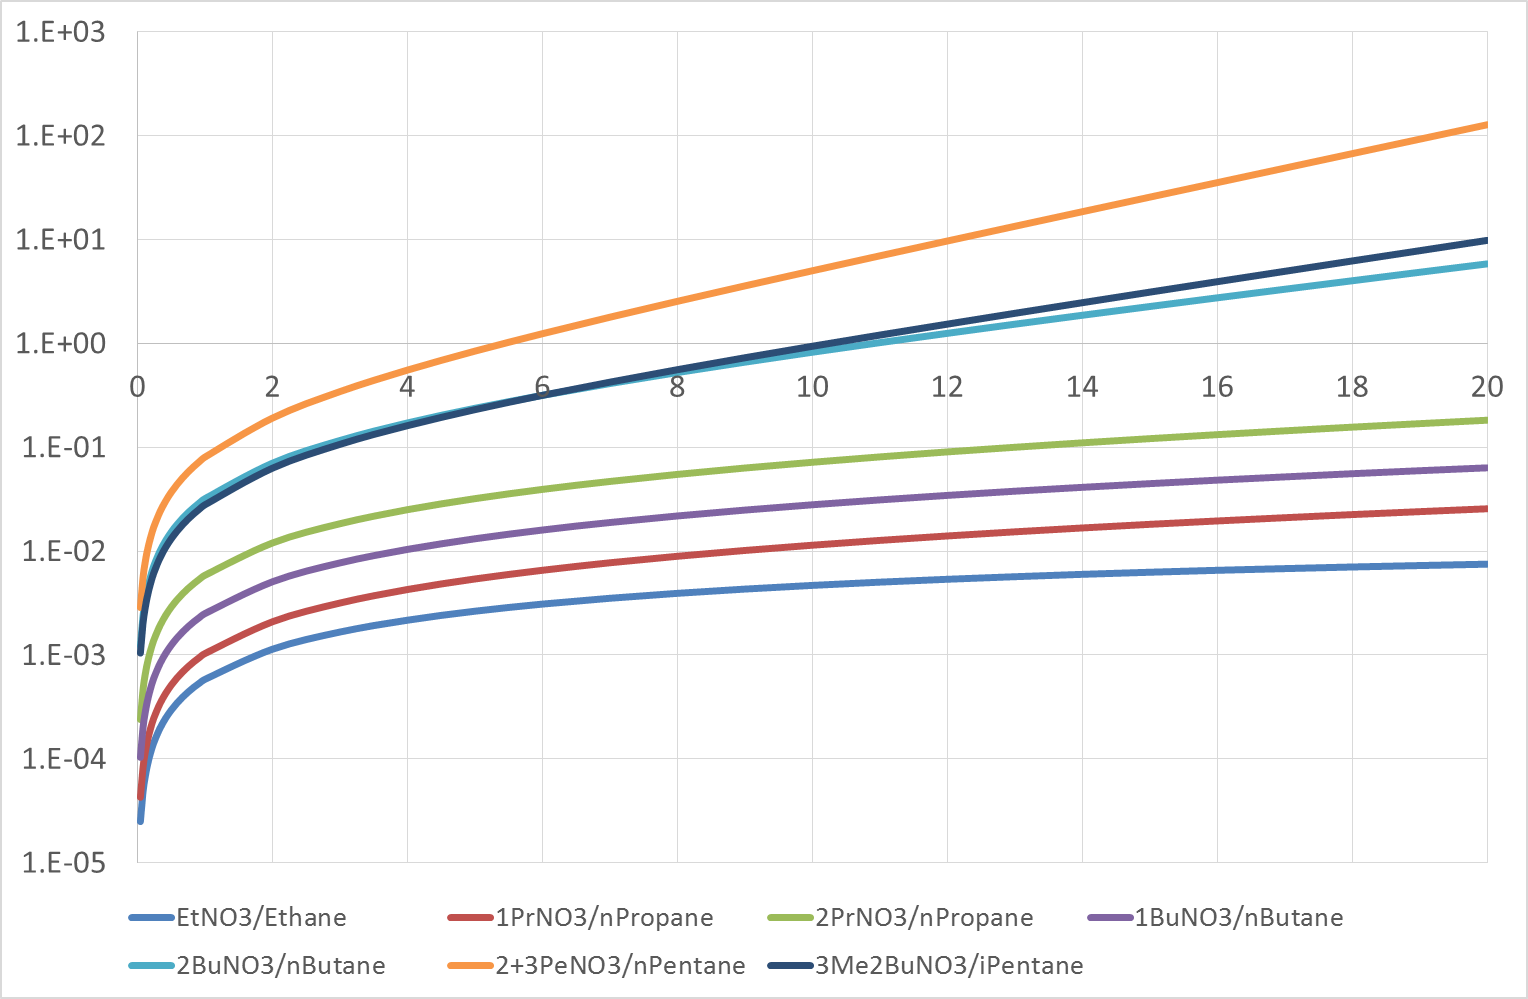
\includegraphics[width=\linewidth]{{./myfigs/1}.png}
		\caption{The time variation of the ratios between alkyl nitrates and their parent hydrocarbons calculated in the 'base' experiment}
		\label{fig:ratio_curves}
\end{figure}

Three modelling experiments are carried out. The first, `base', is designed to simulate a situation when there is no background concentration of the alkyl nitrates (eq. \eqref{eq:model}), which allows us to see how the $[RONO_2]/[RH]$ ratio changes over time following a pulse influx of hydrocarbon. In the second experiment we are trying to take into account an additional source of the alkyl nitrates and their parent hydrocarbons, for which purpose we use a very small typical value (0.1\%, i.e. 0.001) for all their initial ratios. The third experiment is intended to model a situation when the peroxy radical self-reactions ( $ROO\bullet+R'OO\bullet$)  are competitive with the reaction of $ROO\bullet$ and $NO$. It is achieved by using the full equation (eq. \eqref{eq:integral}) till the day 3 inclusively, but then $\beta$ coefficient is assigned to zero implying a cessation of the $ROO\bullet+NO$ reaction, which at once stops the formation of alkyl nitrates.

Figure \ref{fig:ratio_curves} shows the time series of $[RONO_2]/[RH]$ ratios in the `base' experiment conducted for 7 different parent alkanes. It demonstrates that all ratios rapidly increase at the beginning, and after approximately 3 days the growth slows down. This means that at the beginning hydrocarbons are converted to alkyl nitrates more efficiently, but as fewer hydrocarbons remain in the air fewer alkyl nitrates are formed. The relative position of the kinetic curves could be explained by different relative lifetimes of the species. Generally, the longer-chained hydrocarbons have longer lifetime than the shorter-chained ones, the same is true for alkyl nitrates. That is why the lowest curve corresponds to the ratio between the ethyl nitrate and ethane and the highest to the ratio between the sum of 2-pentil nitrate and 3-pentil nitrate and n-pentane.

Following the recommendations from \citep{Bertman1995} the ratios of the alkyl nitrates to their parent hydrocarbons are plotted against the ratio of 2-butyl nitrate to n-butane in order to compare modelling results with the observational data (Fig. \ref{fig:res0}). Generally, the observed data from different campaigns agree reasonably well with the kinetic curves. The relative positions of the data points from four campaigns reflect different ages of sampled air. NAMBLEX data include information about the air experienced photochemical processing in a range from less than 1 day to more than 20 days, ITOP and TORCH2 data range is from less than 1 day to nearly 20 days, and TORCH1 covers photochemical ages from 3 hours to 1 day. Data from the aircraft campaign (ITOP) spans to a greater extent along the kinetic curve, enabling to analyse these data over a wider range of photochemical ages compared to the ground-based observations.

Fig. \ref{fig:res0} also contains the results of the second and third modelling experiments, and shows the sensitivity of the 'base' model to the inclusion of the changes in initial conditions and to the tuning of one of the key model parameters ($\beta$). The discussion of these results is presented in the following section.  

\begin{figure}[h!]
	\centering
	\begin{subfigure}[t]{0.45\textwidth}
		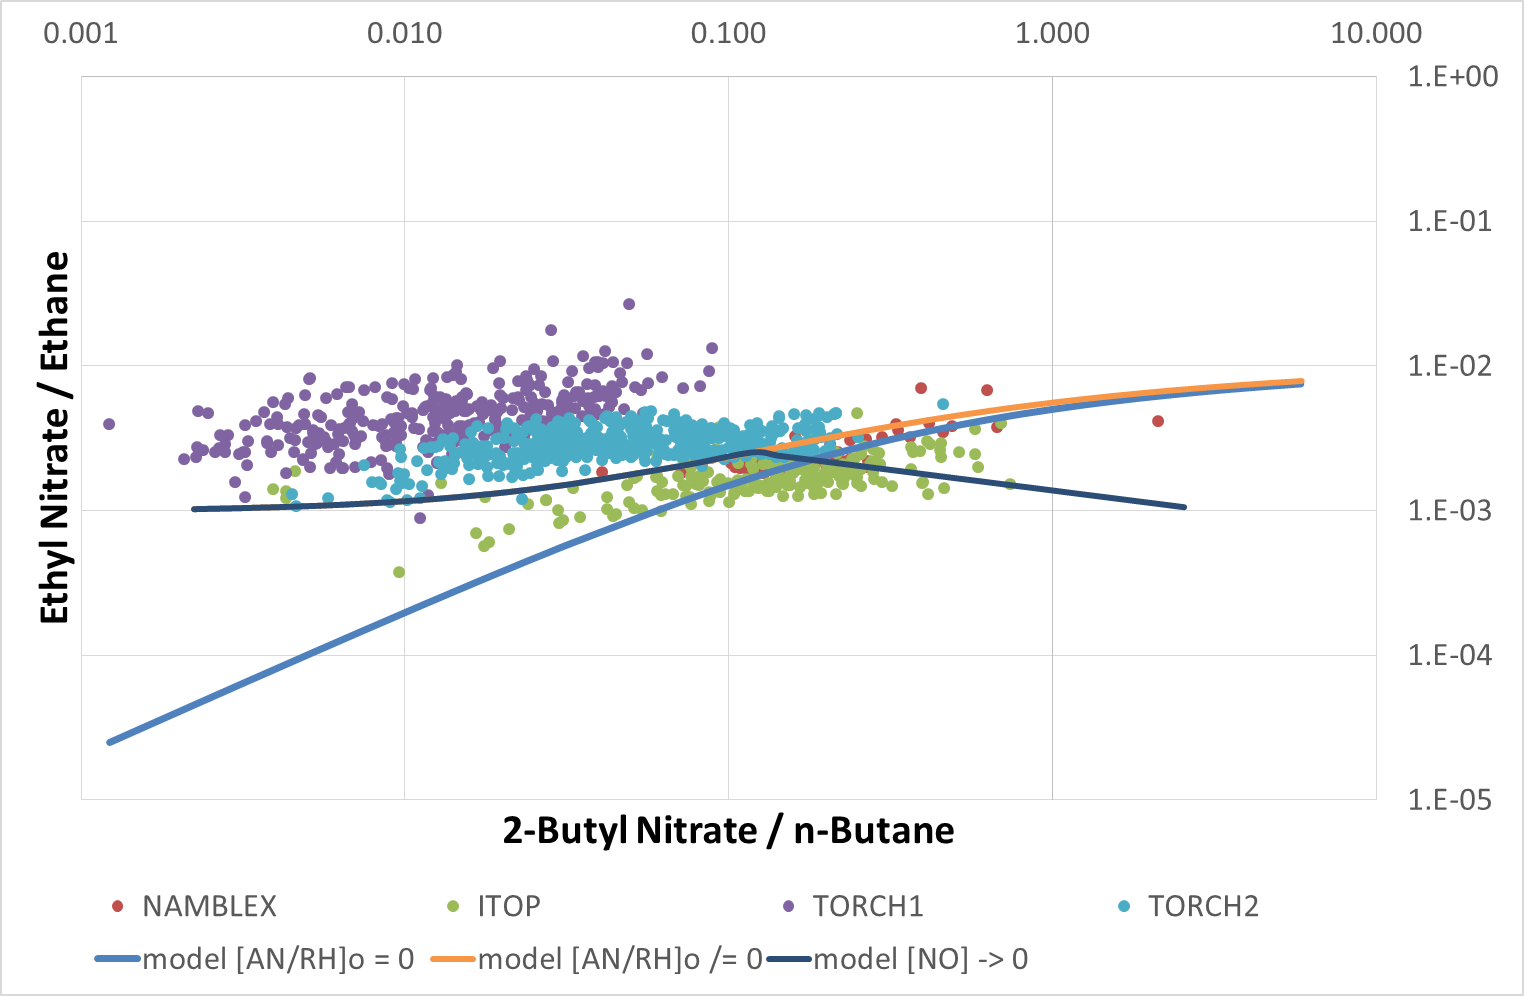
\includegraphics[width=\linewidth]{{./myfigs/2}.png}
		\caption{Ethyl nitrate / ethane}
        \label{fig:res1}
	\end{subfigure}
	\hfill
	\begin{subfigure}[t]{0.45\textwidth}
		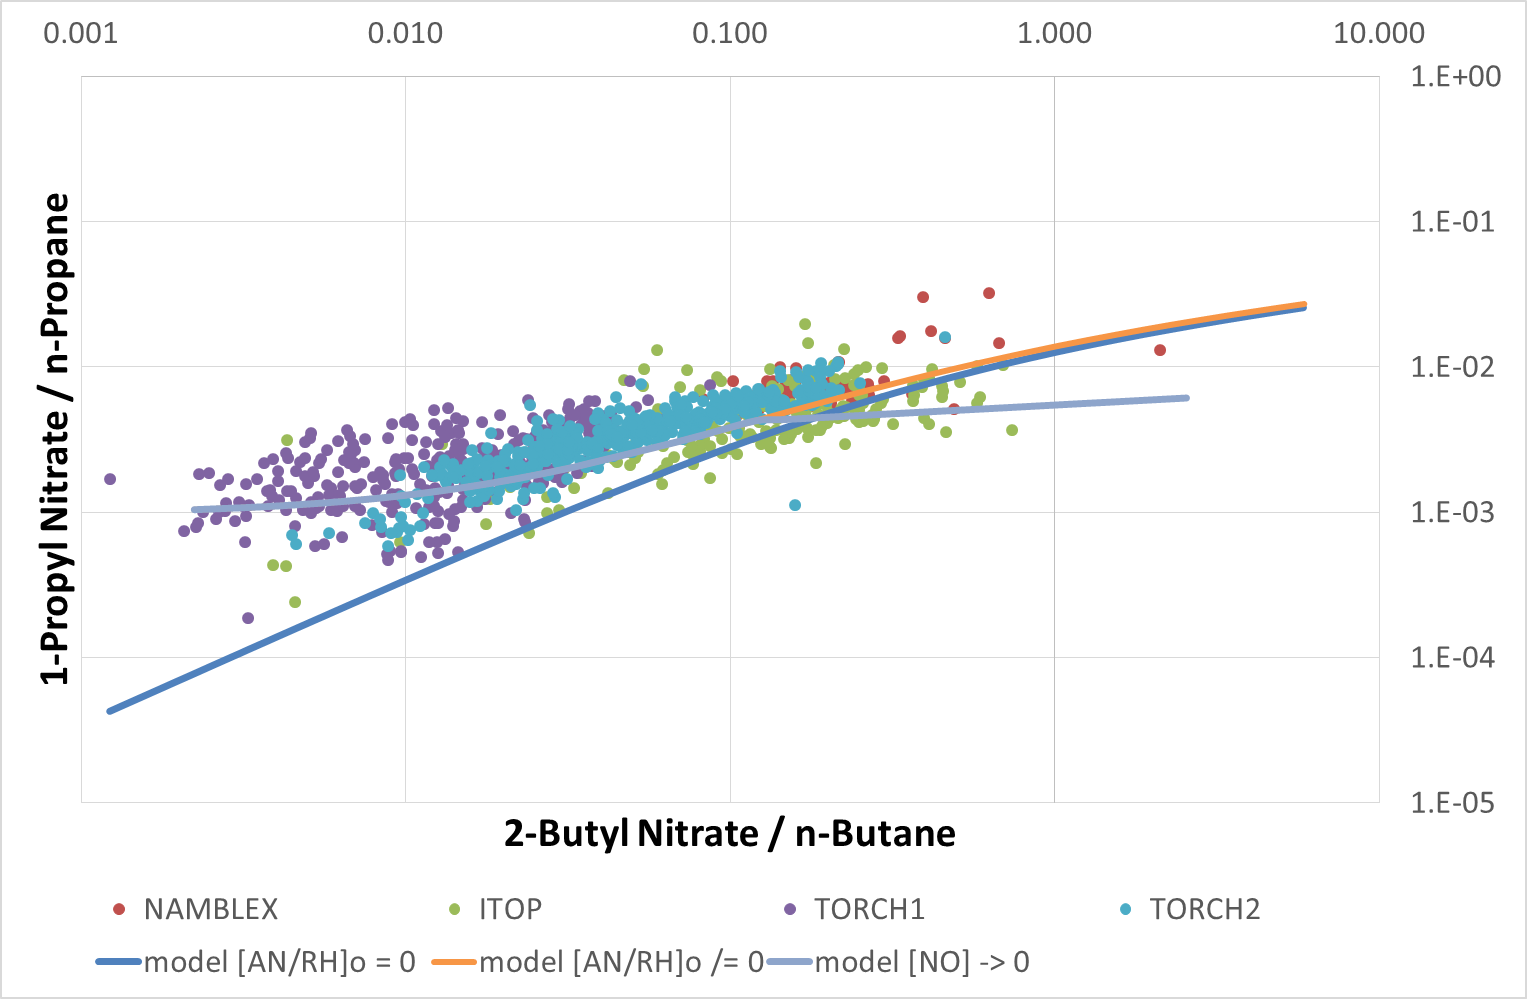
\includegraphics[width=\linewidth]{{./myfigs/3}.png}
		\caption{1-Propyl nitrate / n-propane}
		\label{fig:res2}
	\end{subfigure}
	\hfill
	\begin{subfigure}[t]{0.45\textwidth}
		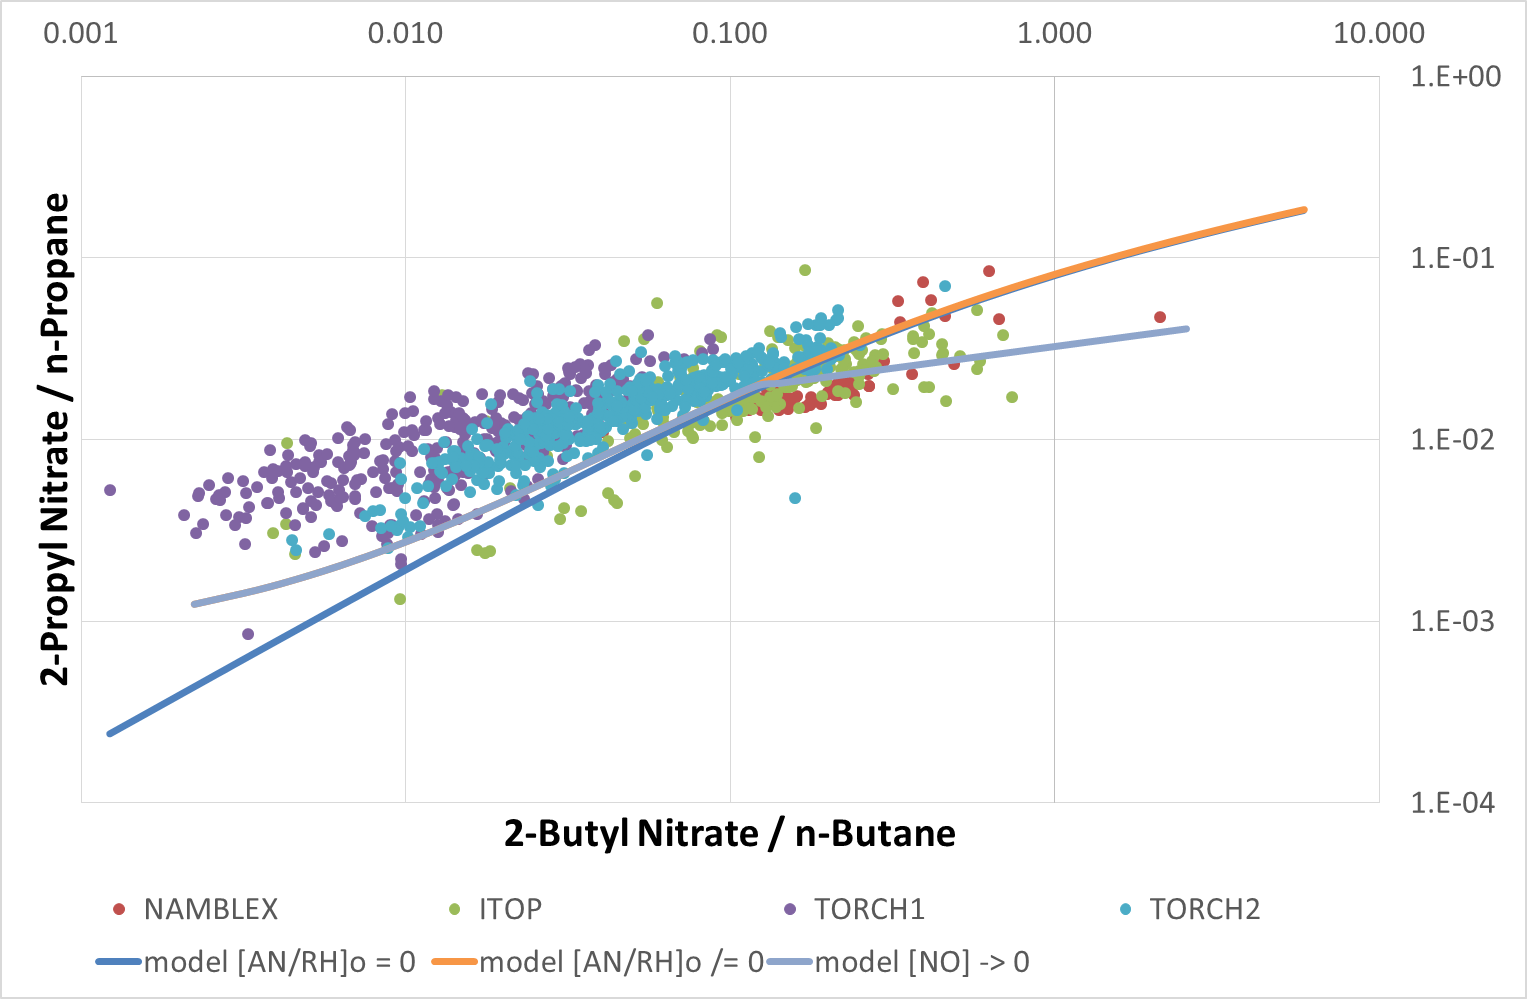
\includegraphics[width=\linewidth]{{./myfigs/4}.png}
		\caption{2-Propyl nitrate / n-propane}
        \label{fig:res3}
	\end{subfigure}
	\hfill
	\begin{subfigure}[t]{0.45\textwidth}
		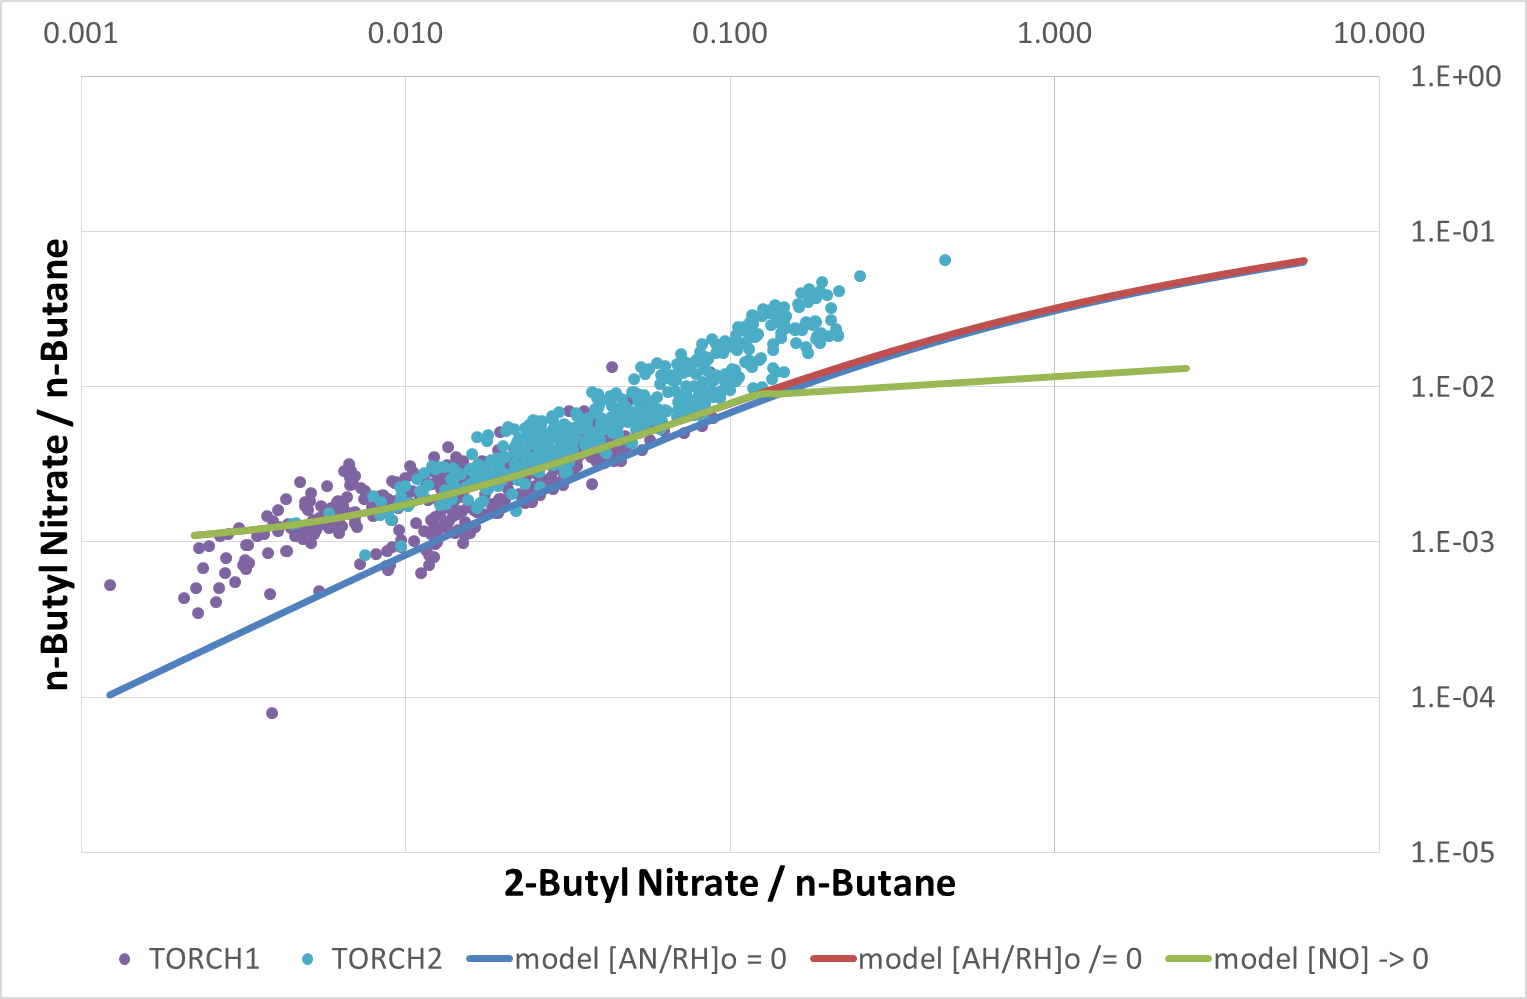
\includegraphics[width=\linewidth]{{./myfigs/5}.png}
		\caption{n-Butyl nitrate / n-butane}
		\label{fig:res4}
	\end{subfigure}
	\hfill
	\begin{subfigure}[t]{0.45\textwidth}
		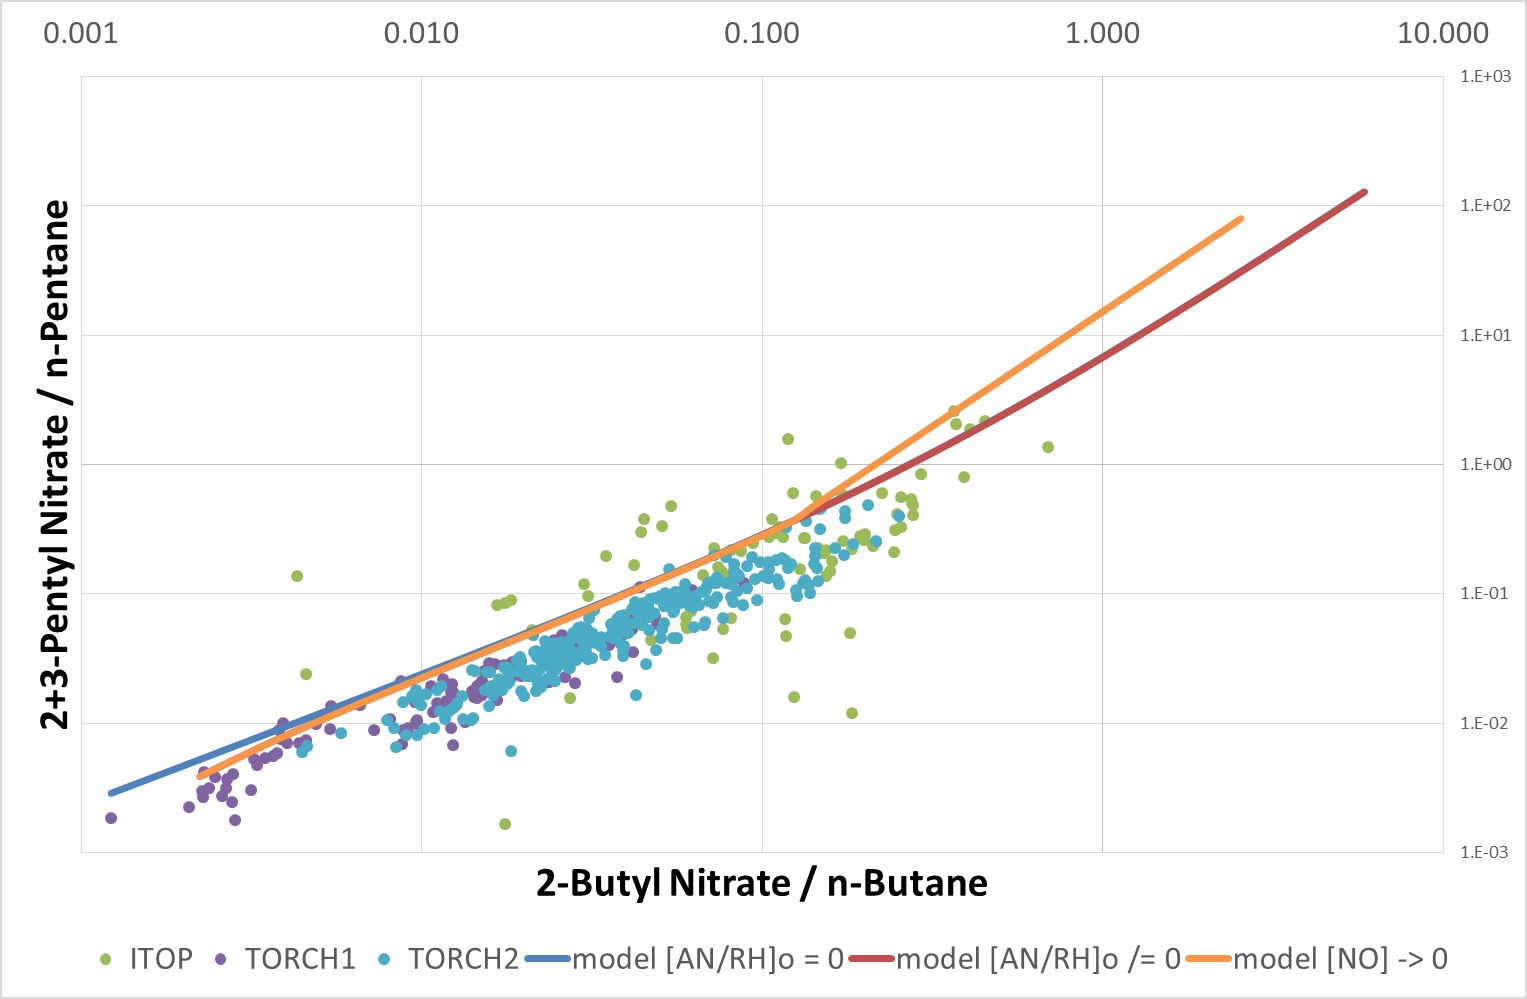
\includegraphics[width=\linewidth]{{./myfigs/6}.png}
		\caption{2+3-Pentyl nitrate / n-pentane}
        \label{fig:res5}
	\end{subfigure}
	\hfill
	\begin{subfigure}[t]{0.45\textwidth}
		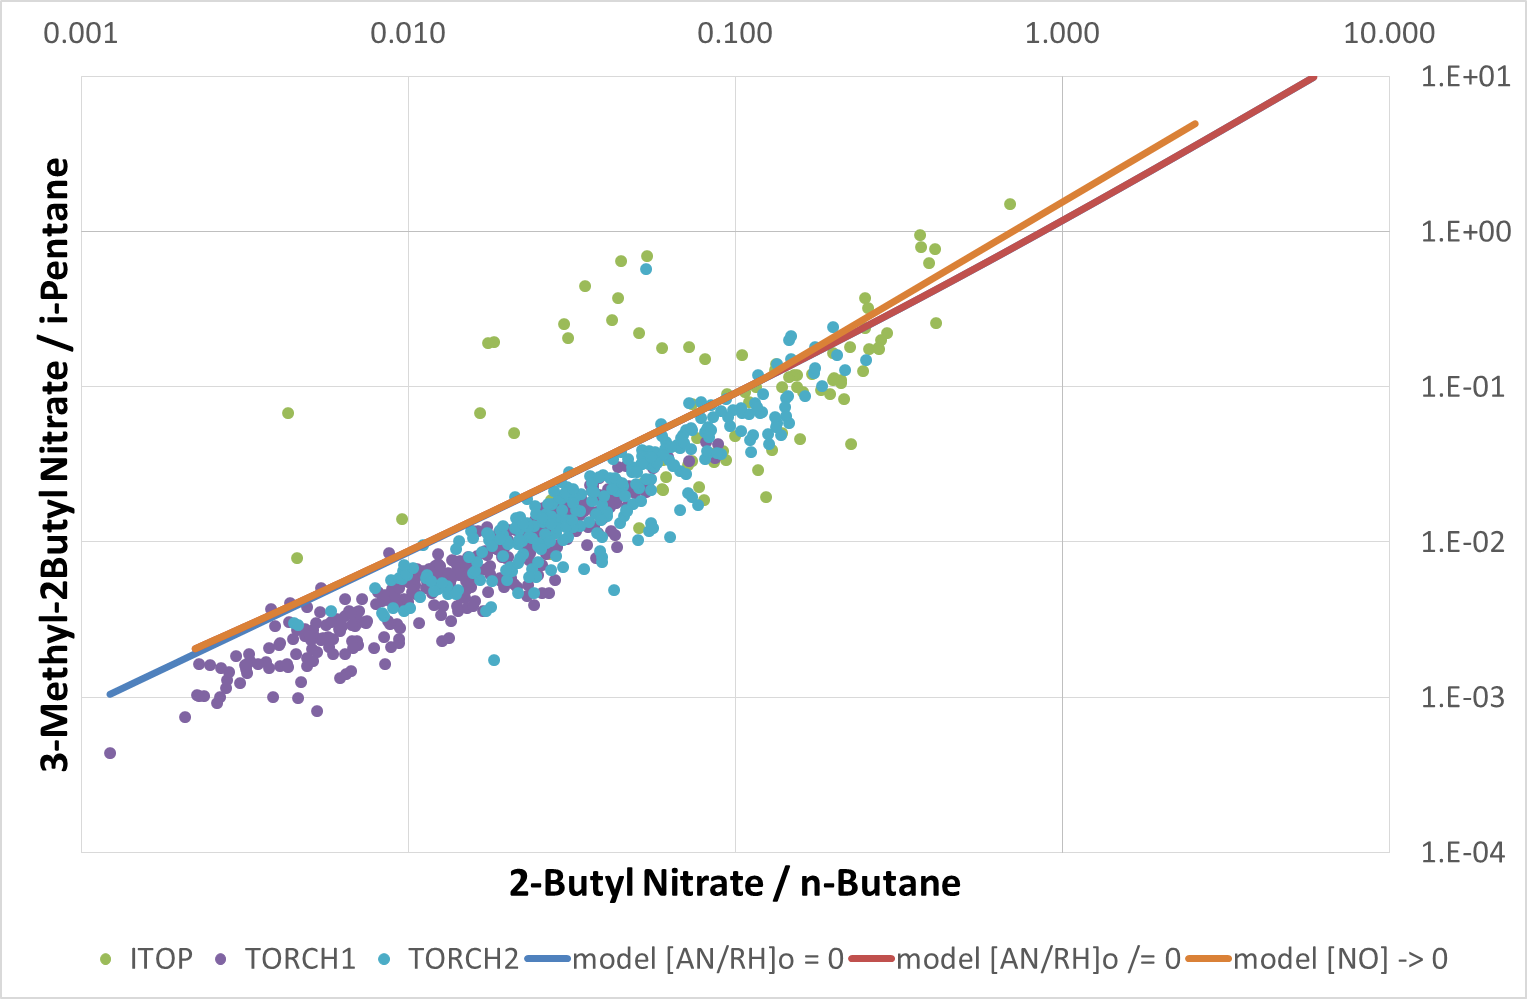
\includegraphics[width=\linewidth]{{./myfigs/7}.png}
		\caption{3-Methyl-2-butyl nitrate / i-pentane}
		\label{fig:res6}
	\end{subfigure}
	\hfill
	\caption{Various $[RONO_2]/[RH]$ ratios plotted against the 2-butyl nitrate/n-butane ratio. The axes are in logarithmic scale. Markers in different colours correspond to the four observational datasets. The lines show the results of the three model runs.}
	\label{fig:res0}
\end{figure}

\section{Discussion} \label{sec:discuss}
The experimental results presented in the previous section provide an opportunity to speculate about the behaviour of our simple model of alkyl nitrate production and loss with time in comparison with the observational data. One of the features that stands out in Fig. \ref{fig:res0} is that the observed ratios of alkyl nitrates to their parent hydrocarbons plotted against the ratio of 2-butyl nitrate to n-butane do not perfectly fit the theoretical curves. The reasons for this discrepancy and how it varies in the datasets from different campaigns are of great interest to us and below we are trying to explain them.

\subsection{Short-chained alkyl nitrates} \label{sec:short_an}
\subsubsection{Short photochemical processing times} \label{sec:short_an_short_time}
Considering  the ratios of ethyl and 1-propyl nitrates, we see that many of the observed data points are scattered above the theoretical curve, especially those corresponding to less photochemically processed air. As other studies show, it could be explained by the existence of an additional source of these alkyl nitrates other than their parent hydrocarbons \citep{Bertman1995, Roberts1998, Stroud2001}. Since ethyl and 1-propyl nitrates strongly correlate with each other and their ratios also exhibit a quite high correlation as well \citep{Reeves2007},  there might be either a common precursor of all four these species, or this might reflect the situation when the fragmentation of longer-chained  hydrocarbons into a number of smaller peroxy radicals takes place eventually leading to the formation of shorter-chained alkyl nitrates. A similar situation occurs with 2-propyl nitrate, which is consistent with the other studies  \citep{Bertman1995, Roberts1998, Stroud2001, Simpson2003}.

The highest deviations from the theoretical curve correspond to the data from TORCH1 campaign. Theoretically it means that air collected during this campaign was sampled from freshly polluted air masses. Indeed, the measurement site of this campaign was located approximately 25 miles to the north-east of central London which in combination with the prevailing south-westerly winds should have resulted in higher concentrations of alkyl nitrates and their parent hydrocarbons. A curve showing modelling result that accounts for this effect is added to the three corresponding plots. As it is seen, the inclusion of non-zero initial concentrations of these species significantly improves the capacity of our model to capture variations in observational data. It is worth noting that this might be an indication of a primary source of these alkyl nitrates \citep{Bertman1995}, and it is congruous with the hypothesis of the short-chained nitrates having  a lifetime long enough to have a significant background concentration.

\subsubsection{Long photochemical processing times} \label{sec:short_an_long_time}
At longer photochemical processing times the ratios of ethyl, 1-propyl and 2-propyl nitrates to their parent hydrocarbons are, on the contrary, often below the theoretical curves. This is because the eqs. \eqref{eq:integral} and \eqref{eq:model} assume $NO$-rich atmosphere therefore excluding $ROO\bullet$ self-reactions and making the reaction \eqref{eq:an_form_loss1} the determining step for the alkyl nitrate formation. To improve the model fit the coefficient $\beta$ in eq. \eqref{eq:integral} has been set to zero after 3 days of photochemical processing, and one more model line is added to the graphs. The fact that the observational data points tend to be scattered around the new model line means that reality is somewhere in between.

\subsubsection{Mixing} \label{sec:short_an_mixing}
One of the key assumptions made in the eq. \eqref{eq:integral} implies that air parcel mixing with the surrounding atmosphere is ignored. It is not a realistic assumption (especially for short-chained species) because in the event of entrainment of older (more photochemically processed) air the ratio of short-chained alkyl nitrates to parent hydrocarbons will in fact decrease and will not be constant. Therefore, mixing could explain some of the points of ethyl nitrate/ethane ratio plotted against 2-butyl nitrate/n-butane ratio being below the theoretical curve at the longer processing times.

For example, this is the case for the data on the measured ratios for ethyl nitrate/ethane and 2-propyl nitrate/propane from TORCH2. The majority of these data points could be identified as less polluted marine air masses that originated in the Arctic before transiting across the North Sea for several days prior to arriving at the site from the North \citep{Worton2010}.

\subsection{Long-chained alkyl nitrates} \label{sec:long_an}
Unlike the short-chained species, the observational data on the long-chained compounds lie below the theoretical curve. This could be explained by the fragmentation of the pentanes into smaller chained alkyl nitrates instead of the pentyl nitrates \citep{Reeves2007}.

\section{Conclusion} \label{sec:conclusion}
In this study a simple model describing the relationship between alkyl nitrates and their parent hydrocarbons is tested against observations. The field data were collected at different sites during different seasons and using various sampling techniques. Covering a wider range of atmospheric conditions the observational data allowed us to test the model more extensively than is usually done in studies based on a particular field campaign. Nevertheless, the theoretical model results agrees well with the alkyl nitrate data, even in case of additional simplifications of equations and the presence of inevitable observational biases. Physically it means that alkyl nitrates (and, therefore, ozone) production indeed had taken place in the air mass, which had been advected from the source region. For instance, the data from TORCH1 campaign showed that the ratios of short-chained alkyl nitrates were higher than in the model owing to the proximity of London as a prominent source of hydrocarbons.

The small values of model departure from the field data indicates that in general the kinetic approach is a robust concept in the alkyl nitrate studies. Moreover, tuning the model in a physically valid way can easily improve its performance and account for the change in ambient atmospheric concentrations. 

However, in some cases the discrepancy between the observations and modelling results cannot be easily interpreted. For example, the model underestimation of ethyl0 ethane and 1-propyl/n-propane ratios can be attributed to  the two different reasons: the presence of a common precursor or a result of fragmentation of the long-chained hydrocarbons to short-chained alkyl nitrates. Understanding of this issue requires a more complex model.

\bibliography{AlkylNitrate_refs}

\end{document}